\documentclass[a4paper,11pt,UTF8]{article}
\usepackage{ctex}
\usepackage{amsmath,amsthm,amssymb,amsfonts}
\usepackage{amsmath}
\usepackage[a4paper]{geometry}
\usepackage{graphicx}
\usepackage{microtype}
\usepackage{siunitx}
\usepackage{booktabs}
\usepackage[colorlinks=false, pdfborder={0 0 0}]{hyperref}
\usepackage{cleveref}
\usepackage{esint} 
\usepackage{graphicx}
\usepackage{ragged2e}
\usepackage{pifont}
\usepackage{extarrows}
\usepackage{mathptmx}
\usepackage{float}
\usepackage{caption}
\usepackage{multirow}
\usepackage{subfigure}
\usepackage{titlesec}
\usepackage{makecell}
\usepackage{tabularx}
\usepackage{graphicx}

\numberwithin{equation}{subsection}
\titleformat{\section}{\Large\bfseries}{\thesection}{1em}{}
\titleformat{\subsection}{\large\bfseries}{\thesubsection}{1em}{}
\titleformat{\subsubsection}{\normalsize\bfseries}{\thesubsubsection}{1em}{}
\begin{document}
\title{\huge 实验报告 \\ 音响放大器的设计}
\author{电子信息与通信学院 \\ 提高2301班 \\ 张禹阳 \ U202314270}

\maketitle

\begin{figure}[H]
	\centering
	\subfigure{
		
\includegraphics[scale=1]{hust.png}
	}
	\subfigure{
		
\includegraphics[scale=1]{eic.png}
	}
\end{figure}

\tableofcontents\newpage

\section{实验名称}
音响放大器的设计
\section{实验目的}
\begin{itemize}
	\item 音响放大器的基本组成
	\item 音调特性控制方法与实现原理
	\item 了解集成功率放大器内部电路工作原理,掌握其外围电路的设计与主要性能参数的测试方法
	\item 掌握音响放大器的设计方法与电子线路系统的装调技术---综合运用所学知识,进行小型多级电子线路系统的设计与装调
\end{itemize}
\section{实验元器件}

\begin{table}[H]
	\centering
	\begin{tabular}{|p{0.25\textwidth}|p{0.25\textwidth}|p{0.25\textwidth}|}
		\hline
		名称 & 型号/参数 & 数量\\
		\hline
		\multirow{2}{*}{集成功放} & LM386
		 & 3\\
		 \cline{2-3}
		& NE5532 & 3\\
		\hline
		\multirow{6}{*}{电阻} & 10$\mathrm{k\Omega}$ & 5 \\
		\cline{2-3}
		 & 13$\mathrm{k\Omega}$ & 1 \\
		\cline{2-3}
		 & 30$\mathrm{k\Omega}$ & 2 \\
		\cline{2-3}
		 & 47$\mathrm{k\Omega}$ & 3 \\
		\cline{2-3}
		 & 75$\mathrm{k\Omega}$ & 1 \\
		\cline{2-3}
		 & 10$\mathrm{\Omega}$ 2W & 1 \\
		\hline
		\multirow{7}{*}{电容} & 0.01$\mu$F & 2 \\
		\cline{2-3}
		& 0.22$\mu$F & 1 \\
		\cline{2-3}
		&0.1$\mu$F & 1 \\
		\cline{2-3}
		& 1$\mu$F & 1\\
		\cline{2-3}
		& 10$\mu$F & 8 \\
		\cline{2-3}
		& 220$\mu$F & 2 \\
		\cline{2-3}
		& 470$\mu$F & 12 \\
		\cline{2-3}
		\hline 	
		\multirow{2}{*}{电位器} & 10$\mathrm{k\Omega}$ & 	3\\
		\cline{2-3}
		& 470$\mathrm{k\Omega}$ & 	2\\
		\hline
		话筒&输出5mV&1\\
		\hline
		音乐播放器&/&1\\
		\hline
	\end{tabular}
\end{table}
\section{实验任务}
设计一个音响
\subsection{功能要求}
具有话音放大、音调控制、音量控制、卡拉OK伴唱等功能(不含电子混响)。
\subsection{已知条件}
\begin{itemize}
	\setlength{\itemsep}{0pt}
	\item 集成功放LM386。
	\item 话筒600$\Omega$,输出信号5mV。
	\item 集成运放NE5532。
	\item 10$\Omega$/2W负载电阻1只。
	\item 8$\Omega$/4W扬声器1只。
	\item 音源(MP3 or PC)。
	\item 电源电压±9V(双电源)。	
\end{itemize}
\subsection{技术指标要求}
\begin{itemize}
	\setlength{\itemsep}{0pt}	
	\item 额定功率:$P_o\geq0.3$W($\gamma< 3\%$)
	\item 负载阻抗:$R_L=10\Omega$(2W)
	\item 频率响应:$f_L=50$Hz,$f_H=20$kHz
	\item 输入阻抗:$R_i\gg20\mathrm{k\Omega}$
	\item 音调控制特性:1kHz处增益为0dB、125Hz和8kHz处有12dB的调节范围,$A_{VL}=A_{VH}≥20$dB(选做)
	
\end{itemize}
\subsection{测量内容}
\section{实验原理及参考电路}
\subsection{实验电路}
\begin{figure}[H]
	\centering
	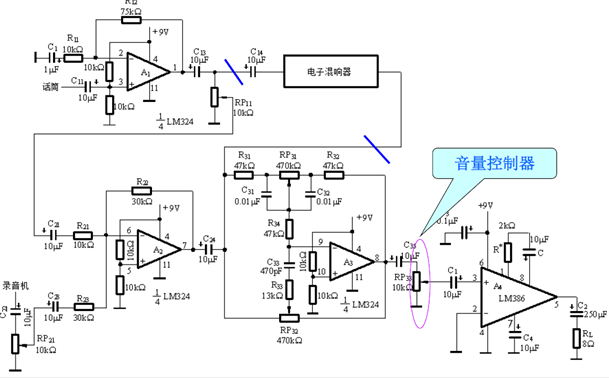
\includegraphics[width=0.7\textwidth]{1.png}
\end{figure}
\subsection{电路安装与调试技术}

\subsubsection{合理布局,分级装调}
\begin{itemize}
	\setlength{\itemsep}{0pt}
	\item 音响放大器是一个小型电路系统,安装前要对整机线路进行合理布局
	\item 一般按照电路的顺序一级一级地布线
	\item 功放级应远离输入级
	\item 每一级的地线尽量接在一起
	\item 连线尽可能短,否则很容易产生自激
	\item 安装前应检查元器件的质量
	\item 安装时特别要注意功放块、运算放大器、电解电容等主要器件的引脚和极性,不能接错
	\item 从输入级开始向后级安装,也可以从功放级开始向前逐级安装
	\item 安装一级调试一级,安装两级要进行级联调试,直到整机安装与调试完成
\end{itemize}
\subsubsection{电路调试技术}
\begin{enumerate}
	\setlength{\itemsep}{0pt}
	\item 电路的调试过程一般是先分级调试,再级联调试,最后进行整机调试与性能指标测试。
	\item 分级调试又分为静态调试与动态调试。
	
	静态调试时,将输入端对地短路,用万用表测该级输出端对地的直流电压。话放、混放、音调电路均由运放组成,若运放是单电源供电,其静态输出直流电压均为\newline VCC/2,功放级输出(OTL电路)也为VCC/2,且输出电容CC两端充电电压也应为\newline VCC/2。若是双电源供电,直流电压均为0。
	动态调试是指输入端接入规定的信号,用示波器观测该级输出波形,并测量各项性能指标是否满足题目要求,如果相差很大,应检查电路是否接错,元器件数值是否合乎要求,否则是不会出现很大偏差的。
	\item 级联调试
	
	单级电路调试时的技术指标较容易达到,但级联后级间相互影响,可能使单级的技术指标发生很大变化,甚至两级不能进行级联。产生的主要原因:一是布线不太合理,形成级间交叉耦合,应考虑重新布线;二是级联后各级电流都要流经电源内阻,内阻压降对某一级可能形成正反馈,应接RC去耦滤波电路。R一般取几十欧姆,C一般用几百微法大电容与0.1F小电容相并联。由于功放输出信号较大,易对前级产生影响,引起自激。集成块内部电路多极点引起的正反馈易产生高频自激,常见高频自激现象如图所示。
	\begin{figure}[H]
		\centering
		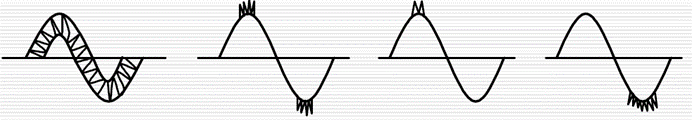
\includegraphics[width=0.9\textwidth]{2.png}
	\end{figure}
	可以加强外部电路的负反馈予以抵消,如功放级①脚与⑤之间接入几百皮法的电容,形成电压并联负反馈,可消除叠加的高频毛刺。
	
\end{enumerate}
\section{实验过程}
\subsection{放大倍数、额定功率及整机效率}
	\begin{figure}[h]
		\centering
		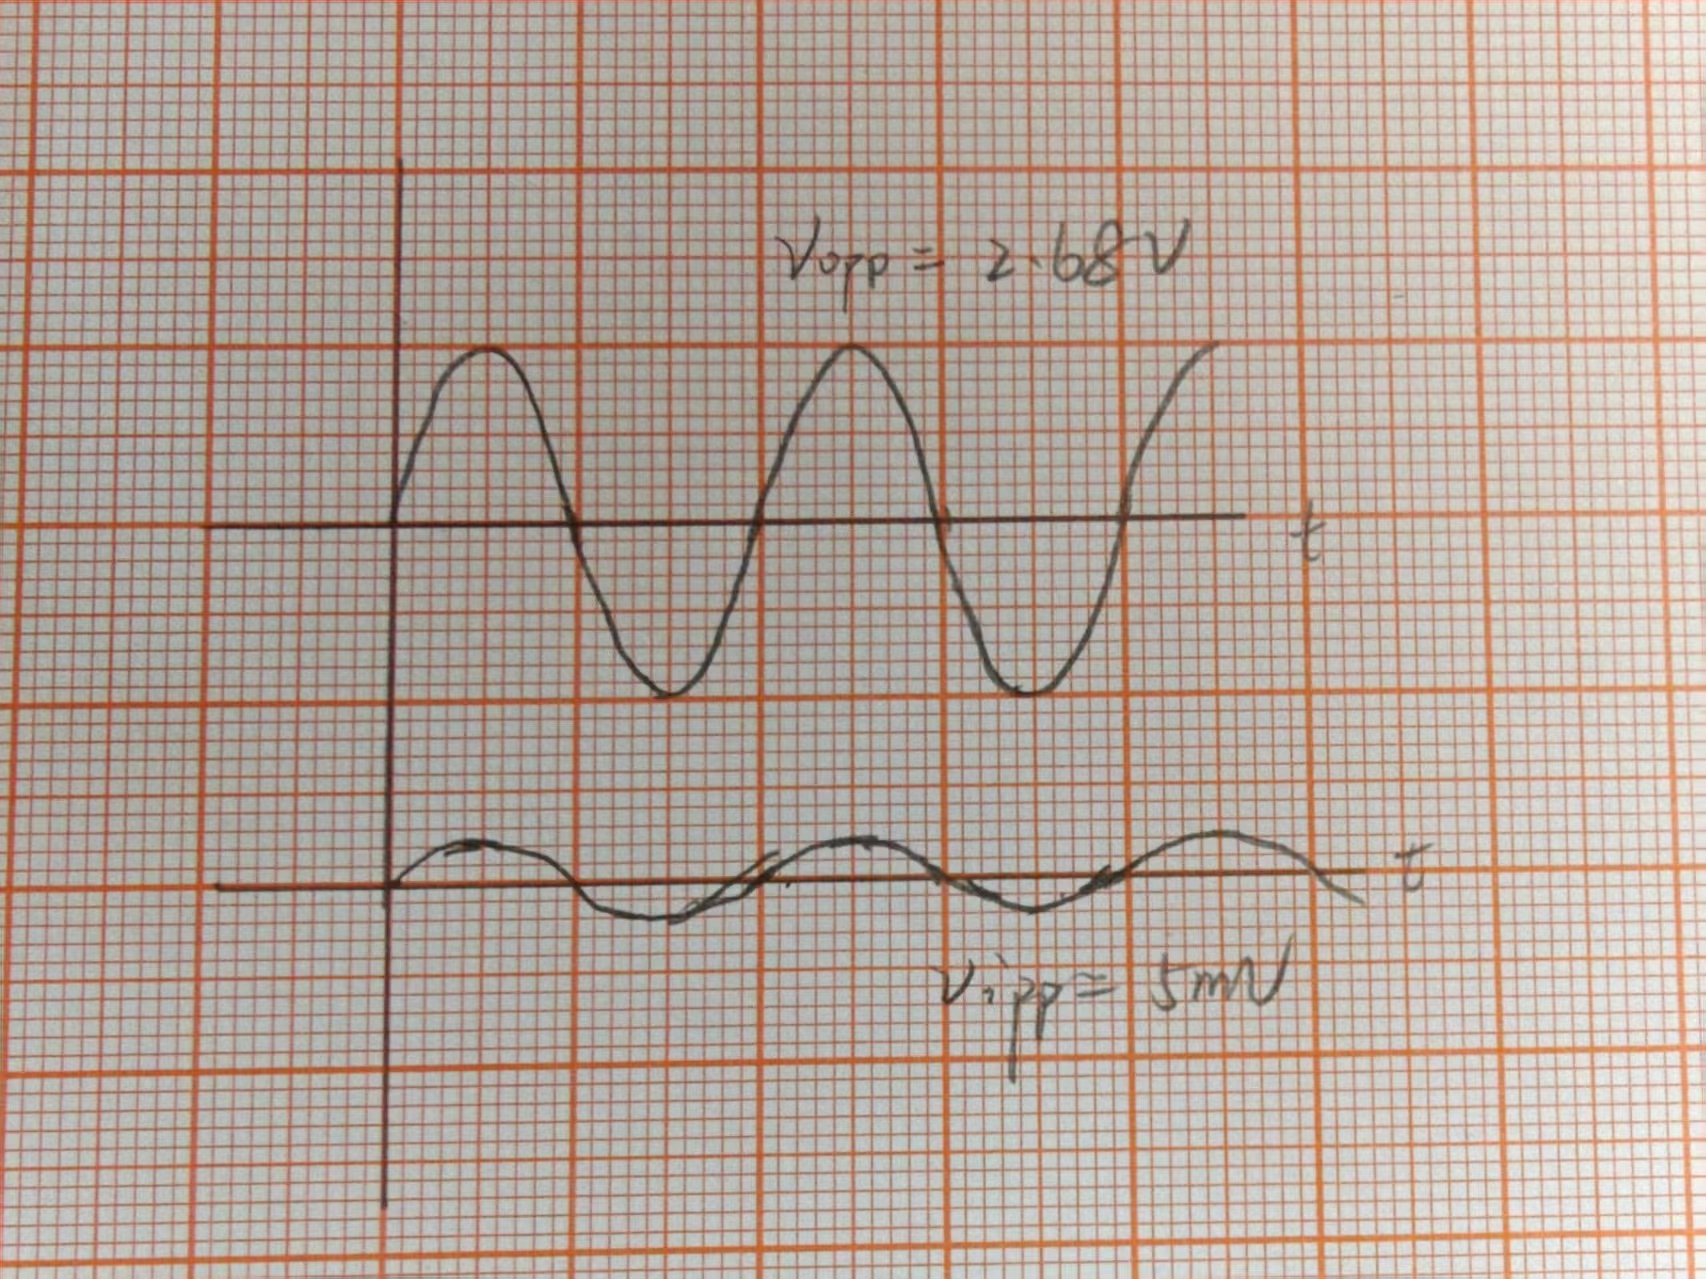
\includegraphics[width=0.8\linewidth]{4.jpg}
	\end{figure}

$A_\mathrm{v}$ = 536

$R_\mathrm{L}$=9.812Ω  $V_\mathrm{o}$=2.68V 

$P_\mathrm{o}=V_\mathrm{o}^{2}/	R_\mathrm{L}$={0.72W}


整机效率 $\eta = \frac{P_o}{P_c} \times 100\% = 45.98\%$

\subsection{输入阻抗}
\begin{figure}[!ht ]
		\centering
		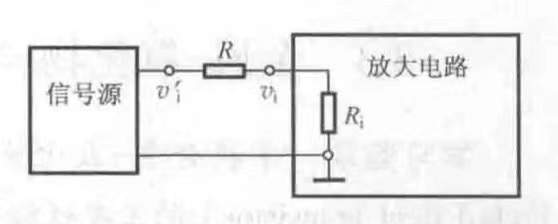
\includegraphics[width=0.8\linewidth]{2.jpg}
		\caption{输入阻抗实验电路图}
\end{figure}
采用在输入回路串入已知电阻的方法测量输入电阻,其局部连接示意图如上图所示。R取值尽量与$R_\mathrm{i}$ 接近(此处取R={100kΩ})。用示波器一通道始终监视輸出	$v_\mathrm{i}$波形,用另一个通道先后測量R接入和不接入时的输出电压	$V_\mathrm{o1}$(测量值为{5.280V})和$V_\mathrm{o2}$(测量值为{2.540V})
则输入电阻为
$R_\mathrm{i} =V_\mathrm{o2}*R/(V_\mathrm{o1}-V_\mathrm{o2}$={68.3kΩ}  满足输入阻抗要求

\subsection{频率响应}
音响放大器的输入端接 $v_i$,$RP_1$ 和 $RP_2$ 置于中间位置,调整信号发生器的频率,测出负载上对应的输出电压
测量数据如下:

\begin{table}[H]
	\centering
	\begin{tabular}{|c|c|c|c|c|c|c|c|c|c|}
		\hline
		f/Hz& 20 & 40&50&500&100&200&500&600&800\\
		\hline
		$V_\mathrm{O}$/mV& 4.120 & 4.880&5.040&5.200&5.280&5.280&5.360&5.280&5.360\\
		\hline
		f/Hz& 1K& 5k&10k&20k&30k&40k&45k&50k&100k\\
		\hline
		$V_\mathrm{o}$/V& 3.201 & 5.280&5.160&5.160&5.040&5.120&5.120&5.080&4.960\\
		\hline
	\end{tabular}
\end{table}

由测量数据可知,$f_\mathrm{L}\approx{40Hz}$,$f_\mathrm{H}>{100kHz}$

\subsection{音调控制特性}
输入信号 $v_i(100\text{mV})$ 从音调控制级输入端的耦合电容加入,输出信号 $v_o$ 从输出端的耦合电容
引出。分别测量低音频提升-高音频衰减和低音频衰减-高音频提升这两条曲线
测量方法如下:将 $RP_1$ 的滑臂置于最左端,$RP_2$ 的滑臂置于最右端,当频率从 20Hz 至 50kHz 变化时
记下对应的电压增益

再将 $RP_1$ 的滑臂置于最右端,$RP_2$ 的滑臂置于最左端,当频率从 20Hz 至 50kHz 变化时
记下对应的电压增益

测量数据如下:

\begin{table}
	\centering
	\begin{tabular}{|c|c|c|c|c|c|c|c|c|c|}
		\hline
		f/Hz & 20 & 50 & 125 & 500&1k&2k&8k&20k&50k \\
		\hline
		$v_o/\text{mV}$&707&460&248&110&101&83&42&20&13 \\
		\hline
		$A_v/\text{dB}$&16.99&13.26&7.89&0.83&0.09&-1.62&-7.54&-13.98&-17.72\\
		\hline
		$v_o/\text{mV}$&11&21&47&94&113&158&470&832&1025 \\
		\hline
		$A_v/\text{dB}$&-19.17&-13.56&-6.56&-0.54&1.06&3.97&13.44&18.39&20.21\\
		\hline
	\end{tabular}
\end{table}

绘制得到的音调控制特性曲线如下:
\begin{figure}
	\centering
	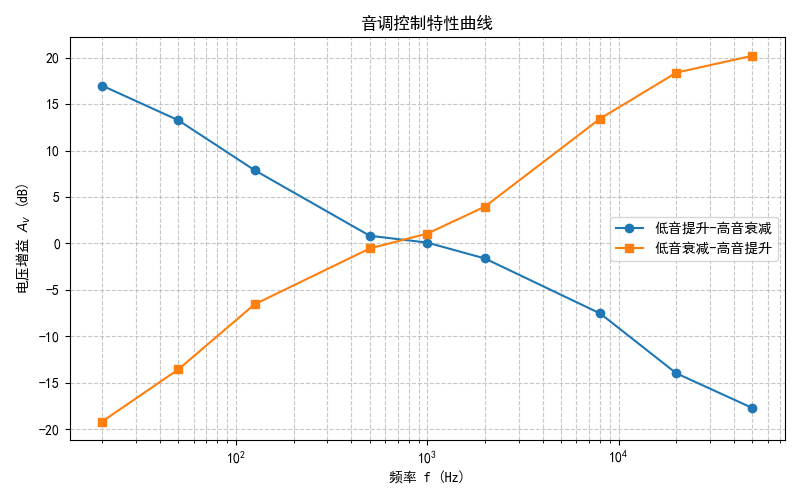
\includegraphics[width=0.8\linewidth]{5.png}
\end{figure}


\section{实验小结}
本次实验规模较大,虽然搭建较快,但是调试耗费了非常多的时间。总体来说整个过程非常艰辛,但尝试多次后还是
得到了最终结果。本次实验中我更加深入理解了运算放大电路的级联,各级之间
保持怎么样的输出输出,分别实现怎么样的功效等。
\end{document}